


\section{Library Evaluation}

This section presents the evaluation results of the TAkka library.  
We show that the Wadler's type pollution problem can be avoided 
in a straightforward way by using TAkka. We further assess the TAkka library by 
porting examples written in Erlang and Akka.  Results show that TAkka 
detects type errors without causing obvious runtime and code-size overheads.



\subsection{Wadler\rq{}s Type Pollution Problem}
\label{type_pollution}

Wadler\rq{}s type pollution problem refers to the situation where a
communication interface of a component publishes too much type information to 
another party and consequently that party can send the component a message not
expected from it.  Without due care, actor-based systems constructed using the
layered architecture or the MVC model \begin{comment}citation? MVC is a 
well-known model\end{comment} 
can suffer from the type pollution problem.

One solution to the type pollution problem is using separate channels for
distinct parties.  Programming models that support this solution includes the
join-calculus \citep{full_join} and the typed $\pi$-calculus \citep{pi_book}.

TAkka solves the type pollution problem by using polymorphism.  Take the
code template in Figure \ref{MVC} for example. Let {\tt V2CMessage} and {\tt 
M2CMessage} be the type of messages expected from the View and the Model
respectively.  Both {\tt V2CMessage} and {\tt M2CMessage} are subtypes of {\tt
ControllerMsg}, which is the least general type of messages expected by the 
controller. In the template code, the controller publishes itself as different 
types to the view actor and the model actor.  Therefore, both the view and the
model only know the communication interface between the controller and itself.
The {\tt ControllerMsg} is a sealed trait so that users cannot define a 
subtype of 
{\tt ControllerMsg} outside the file and send the controller a message of 
unexpected type.  Although type convention in line 25 and line 27 can be 
omitted, we explicitly use the {\tt publishAs} to express our intention and 
let the compiler check the type.  The code template is used to implement the 
Tic-Tac-Toe example in the TAkka code repository.
\begin{comment}
\mycomment{I failed to found small-sized example that uses layered
architecture.  Therefore, I use the core structure of the Tik-Tak-Tok example
here. I implement the Tik-Tak-Tok example for demonstration purpose. I want
to keep the code size small, but the Tik-Tak-Tok example still has 291 lines of
code.}
\end{comment}



\begin{figure}[h]
\label{MVC}
\begin{lstlisting}
sealed trait ControllerMsg
class V2CMessage extends ControllerMsg
class M2CMessage extends ControllerMsg

trait C2VMessage
case class ViewSetController(controller:ActorRef[V2CMessage]) extends 
C2VMessage
trait C2MMessage
case class ModelSetController(controller:ActorRef[M2CMessage]) extends 
C2MMessage
class View extends TypedActor[C2VMessage] {
  private var controller:ActorRef[V2CMessage]
  // rest of implementation
}
Model extends TypedActor[C2MMessage] {
  private var controller:ActorRef[M2CMessage]
  // rest of implementation
}
class Controller(model:ActorRef[C2MMessage], view:ActorRef[C2VMessage]) extends 
TypedActor[ControllerMessage] {
  override def preStart() = {
    model ! ModelSetController( typedSelf.publishAs[M2CMessage])
    view ! ViewSetController( typedSelf.publishAs[V2CMessage])
  }
  // rest of implementation
}
\end{lstlisting}
\caption{Template for Model-View-Controller}
\end{figure}



\subsection{Expressiveness and Correctness}
\label{expressiveness}
Table \ref{express} lists the examples used for expressiveness and 
correctness.  We selected examples from Erlang Quiviq \citep{quviq}
and open source Akka projects to ensure that the main requirements for actor 
programming are not unintentionally neglected.  Examples from Erlang 
Quiviq are re-implemented using both Akka and TAkka.  Examples from 
Akka projects are re-implemented using TAkka.  Following the suggestion in  
\citep{HePa06}, we assess the overall code modification and code 
size by calculating the geometric mean of all examples. The evaluation results 
in Table \ref{express} show that when porting an Akka program to TAkka, about 
7.4\% lines of code need to be modified including additional type declarations. 
Sometimes, the code size can be smaller because TAkka code does not 
need to handle unexpected messages.  On average, the total program size 
of Akka and TAkka applications are almost the same.

A type error is reported by the compiler when porting the Socko example 
\citep{SOCKO} from its Akka implementation to equivalent TAkka implementation.
SOCKO is a library for building event-driven web services.  The SOCKO designer
defines a {\tt SockoEvent} class to be the supertype of all events.  One
subtype of {\tt SockoEvent} is {\tt HttpRequestEvent}, representing events
generated when an HTTP request is received. The designer further implements
subclasses of {\tt Method}, whose {\tt unapply} method intends to pattern
match {\tt SockoEvent} to {\tt HttpRequestEvent}.  The SOCKO
designer made a type error in the method declaration so that the {\tt unapply}
method pattern matches {\tt SockoEvent} to {\tt SockoEvent}. The type error is
not exposed in test examples because the those examples always passes instances 
of {\tt HttpRequestEvent} to the {\tt unapply} method and send the returned
values to an actor that accepts messages of {\tt HttpRequestEvent} type.
Fortunately, the design flaw is exposed when upgrading the SOCKO implementation 
using TAkka.




\begin{table*}[t]
\begin{center}
\begin{tabular}{| p{2.3 cm} | p{2.3 cm} | c | c |  c | c | c |}
\hline

Source & Example & \specialcell{Akka Code \\ Lines} &
\specialcell{Modified\\ TAkka Lines} & \specialcell{\% of \\Modified Code} &
\specialcell{TAkka Code\\ Lines}
& \specialcell{\% of \\Code Size} \\
\hline
Quviq   & ATM simulator & 1148 & 199 & 17.3 & 1160 & 101 \\
\cline{2-7}
\citep{quviq}                                    & Elevator Controller &
2850 & 172 & 9.3 & 2878 & 101 \\
\hline


                                                               & Ping Pong & 67
& 13 & 19.4 & 67 & 100 \\
\cline{2-7}
Akka Documentation                 & Dining Philosophers & 189 & 23 & 12.1 &
189 & 100  \\
\cline{2-7}
 \citep{akka_doc}             & Distributed Calculator  & 250 &
43 & 17.2 & 250 & 100 \\
\cline{2-7}
                                                     & Fault Tolerance & 274 &
69 & 25.2 & 274 & 100 \\
\hline

                                                    & Barber Shop \citep{BarberShop}& 754 & 104 & 
13.7 & 751 & 99 \\
\cline{2-7}
Other Open Source             & EnMAS \citep{EnMAS} & 1916 & 213 & 11.1 & 1909 &
100 \\
\cline{2-7}
  Akka Applications                & Socko Web Server \citep{SOCKO}  & 5024 & 227
& 4.5 & 5017 & 100 \\
\cline{2-7}
                                                     & Gatling \citep{Gatling}
& 1635 & 111 & 6.8 & 1623 & 99 \\
\cline{2-7}
                                                     & Play Core \citep{play_doc}
& 27095 & 15 & 0.05 & 27095 & 100 \\
\hline
geometric mean                   & & 991.7 & 71.6 & 7.4 & 992.1 & 100.0 \\
\hline
\end{tabular}
% }
\caption{Results of Correctness and Expressiveness Evaluation}
\end{center}
\label{express}
\end{table*}

\begin{comment}
\begin{table*}[t]
\label{efficiency_description}

\begin{center}
\begin{tabular}{| l | p{10.5 cm} |}
\hline

Example & Description \\
\hline
bang & This benchmark tests many-to-one message passing.  The benchmark
spawns a specified number sender and one receiver.  Each sender sends a
specified number of messages to the receiver.\\
\hline
big & This benchmark tests many-to-many message passing.  The benchmark
creates a number of actors that exchange ping and pong messages. \\
\hline
ehb & This is a benchmark and stress test.  The benchmark is
parameterized by the number of groups and the number of messages sent from each
sender to each receiver in the same group. \\
\hline
mbrot & This benchmark models pixels in a 2-D image.  For each pixel,
the benchmark calculates whether the point belongs to the Mandelbrot set. \\
\hline
%parallel & This benchmark spawns a number of processes, where a list of
%N timestamps is concurrently created.  \\
%\hline
%genstress & This benchmark is similar to the bang test.  It spawns an
%echo server and a number of clients.  Each client sends some dummy messages to
%the server and waits for its response.  The Erlang version of this test can be
%executed with or without using the gen\_server behaviour.  For generality, this
%benchmark only tests the version without using gen\_server. \\

%\hline
ran & This benchmark spawns a number of processes.  Each process
generates a list of ten thousand random integers, sorts the list and sends the
first half of the result list to the parent process. \\
\hline
 serialmsg & This benchmark tests message forwarding through a
dispatcher. \\
\hline
\end{tabular}
% }
\caption{Examples for Efficiency and Scalability Evaluation}
\end{center}
\end{table*}


\hline
timer\_wheel & This benchmark is a modification to the big test.  While
responding to ping messages, a process in this message also waits pong messages.
 If no pong message is received within the specified timeout, the process
terminates itself. \\
\end{comment}





\subsection{Efficiency, Throughput, and Scalability}
\label{efficiency}

The TAkka library is built on top of Akka so that code for shared features 
can be re-used.  The three main source of overheads in the TAkka implementation
are: (i) the cost of adding an additional operation layer on top of Akka 
code, (ii) the cost of constructing type descriptors, and (iii) the cost of 
transmitting type descriptor in distributed settings. We assess the upper bound 
of the cost of the first two factors by a micro benchmark which assesses the 
time of initializing {\it n} instances of {\tt MyActor} defined in Figure
\ref{fig:akkastring} and Figure \ref{takkastring}. When {\it n} ranges from 
$10^4$ to $10^5$, the TAkka implementation is about 2 times slower as
the Akka implementation.  The cost of the last factor is close to the cost of
transmitting the string representation of fully qualified type names.



The JSON serialization example \citep{techempower} is used to compare the 
throughput of 4 web services built using Akka Play, TAkka Play, Akka 
Socko, and TAkka Scoko.  For each HTTP request, the example gives an 
HTTP response with pre-defined content.  All web services are deployed to 
Amazon EC2 Micro instances (t1.micro), which has 0.615GB Memory. The throughput 
is tested with up to 16 EC2 Micro instances.  For each number of EC2 instances, 
10 rounds of throughput measurement are executed to gather the average and 
standard derivation of the throughput. The results reported in Figure 
\ref{throughput} shows that web servers built using Akka-based library and 
TAkka-based library have similar throughput.

We further investigated the speed-up of multi-node TAkka applications by 
porting 6 micro benchmark examples, from the BenchErl benchmarks in the RELEASE 
project \citep{RELEASE}.  Each BenchErl benchmark spawns one master process and 
many child processes for a tested task.  Each child process is asked to perform 
a certain amount of computation and report the result to the master process.  
The benchmarks are run on a 32 node Beowulf cluster at the Heriot-Watt 
University. Each Beowulf node comprises eight Intel 5506 cores running at
2.13GHz. All machines run under Linux CentOS 5.5. The Beowulf nodes are
connected with a Baystack 5510-48T switch with 48 10/100/1000 ports.

Figure \ref{runtime} and \ref{scalability} reports the results of the BenchErl 
benchmarks.   We report the average and the standard deviation 
of the run-time of each example.  Depending on the ratio of the computation 
time and the I/O time, benchmark examples scale at different levels.  In 
all examples, TAkka and Akka implementations have almost identical 
run-time and scalability.


\begin{figure}[h]
     \begin{center}
        \subfigure[]{
            \label{fig:play_throughput}
            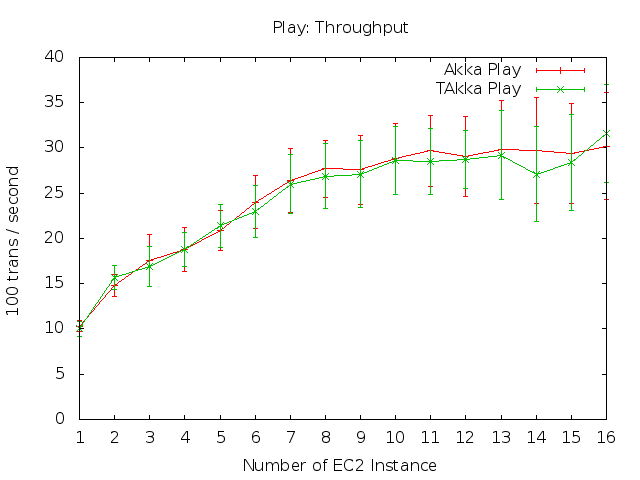
\includegraphics[scale=0.25]{Play_throughput.png}
        }
        \subfigure[]{
           \label{fig:socko_throughput}
           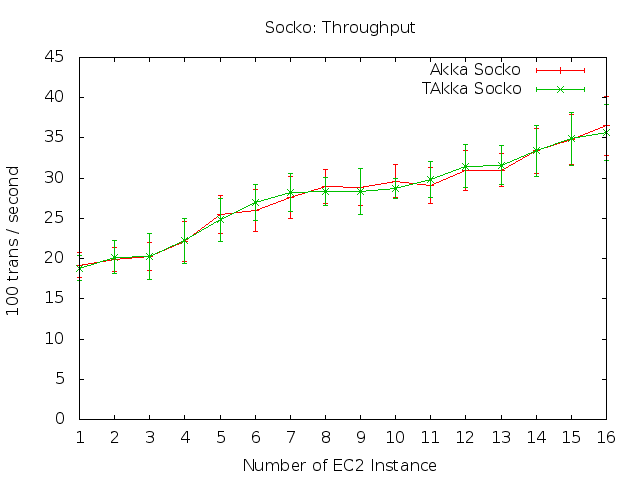
\includegraphics[scale=0.25]{Socko_throughput.png}
        }
    \end{center}
     \caption{Throughput Benchmarks}
   \label{throughput}
\end{figure}

\begin{figure}[p]
     \begin{center}
        \subfigure[]{
            \label{fig:2_1}
            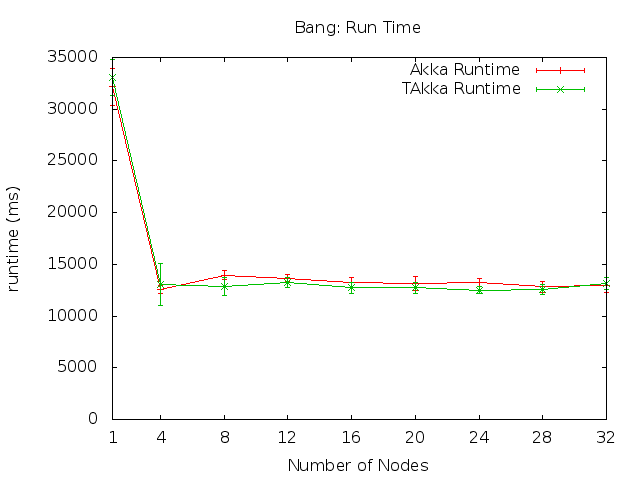
\includegraphics[scale=0.16]{Bang_time.png}
        }
        \subfigure[]{
           \label{fig:2_2}
           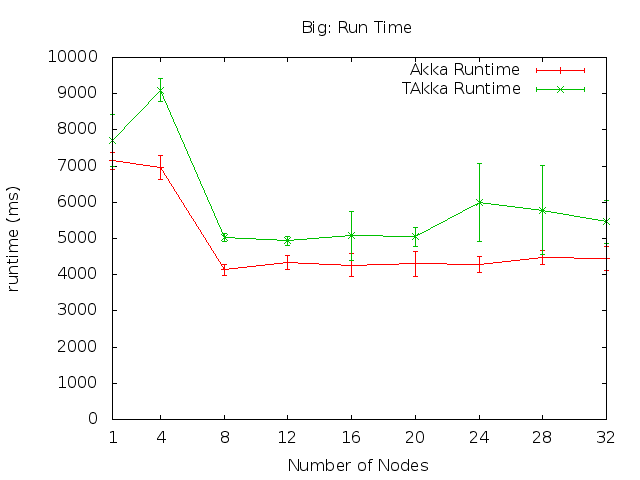
\includegraphics[scale=0.16]{Big_time.png}
        }
        \subfigure[]{
            \label{fig:2_3}
            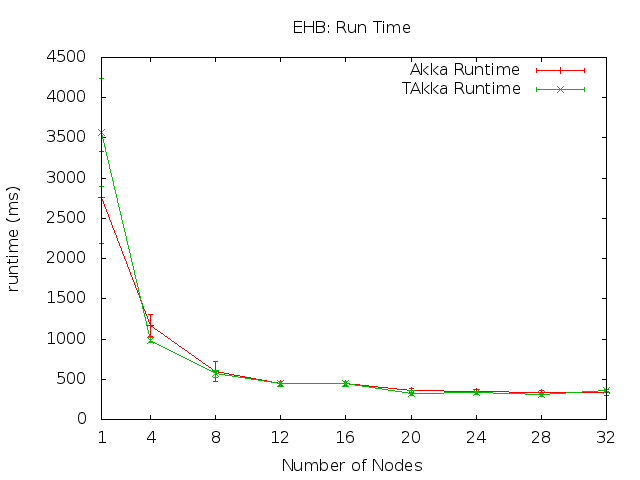
\includegraphics[scale=0.16]{EHB_time.png}
        }\\
        \subfigure[]{
            \label{fig:2_5}
            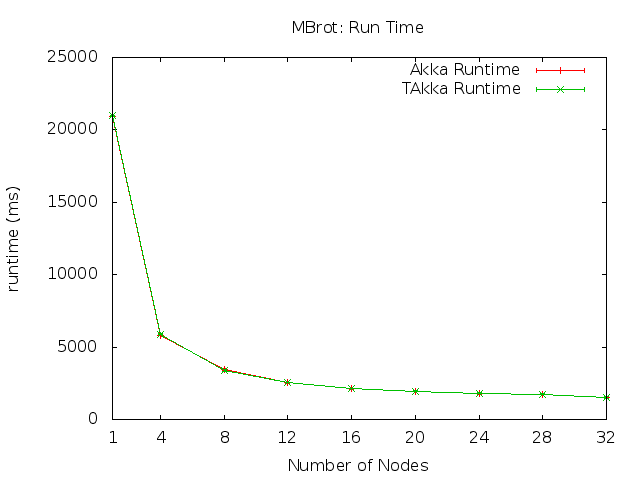
\includegraphics[scale=0.16]{MBrot_time.png}
        }
        \subfigure[]{
            \label{fig:2_7}
            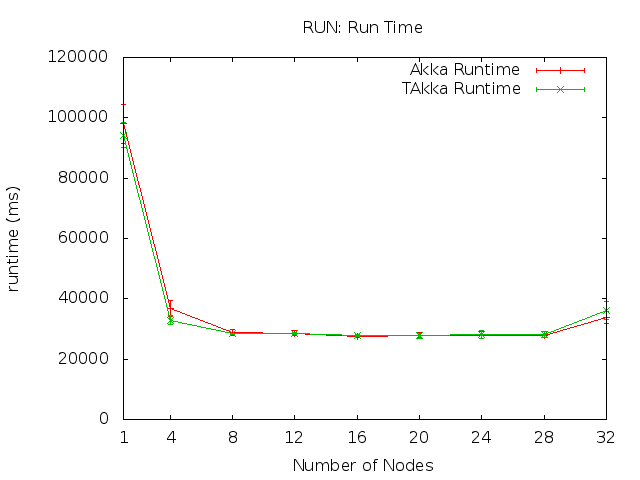
\includegraphics[scale=0.16]{RUN_time.png}
        }
        \subfigure[]{
           \label{fig:2_8}
           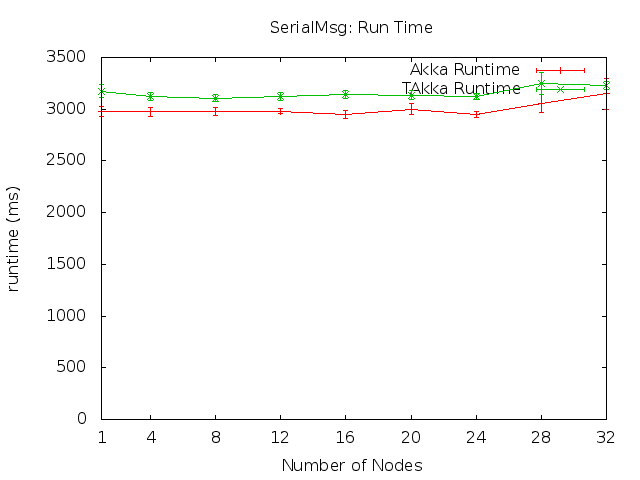
\includegraphics[scale=0.16]{SerialMsg_time.png}
        }\\
    \end{center}
    \caption{Runtime Benchmarks 2}
   \label{runtime}
\end{figure}
\begin{figure}[p]
     \begin{center}
        \subfigure[]{
            \label{fig:2_9}
            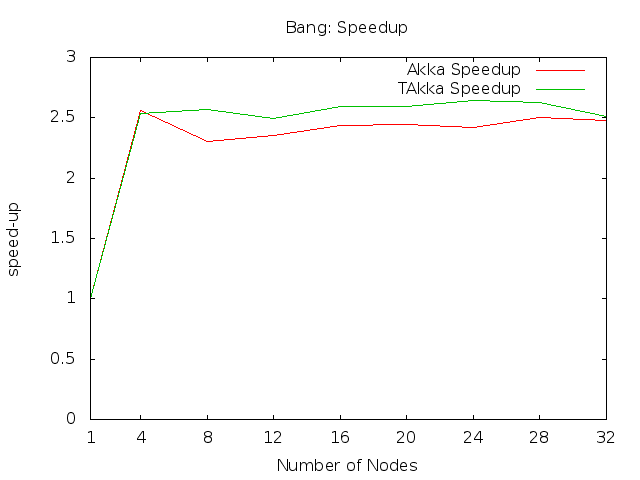
\includegraphics[scale=0.16]{Bang_speedup.png}
        }
        \subfigure[]{
           \label{fig:2_10}
           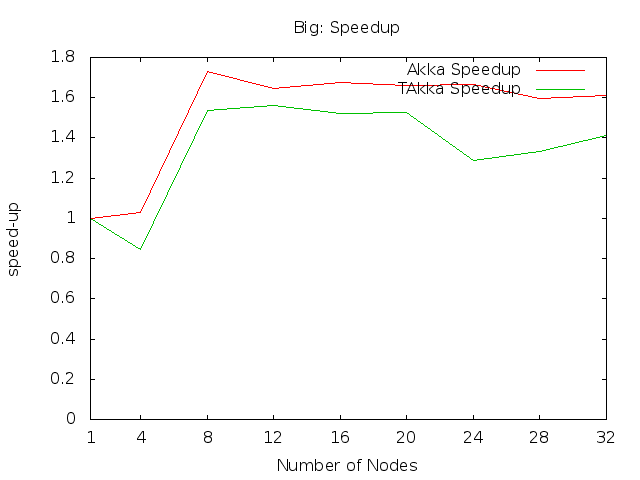
\includegraphics[scale=0.16]{Big_speedup.png}
        }
        \subfigure[]{
            \label{fig:2_11}
            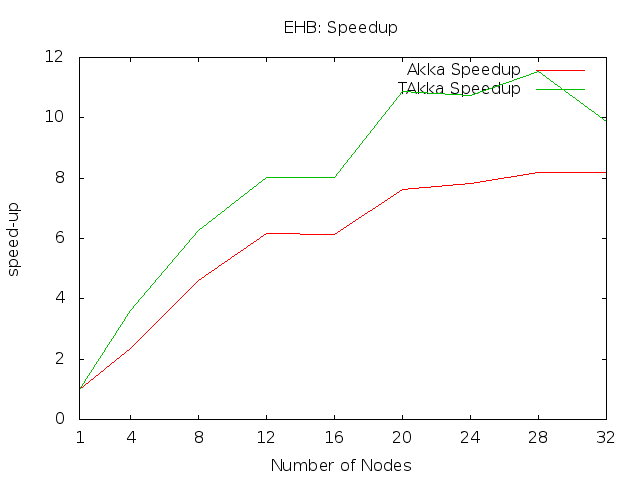
\includegraphics[scale=0.16]{EHB_speedup.png}
        }\\
        \subfigure[]{
            \label{fig:2_13}
            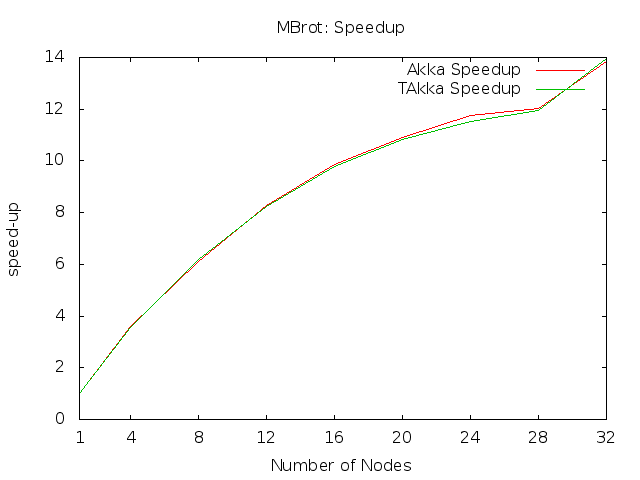
\includegraphics[scale=0.16]{MBrot_speedup.png}
        }
        \subfigure[]{
            \label{fig:2_15}
            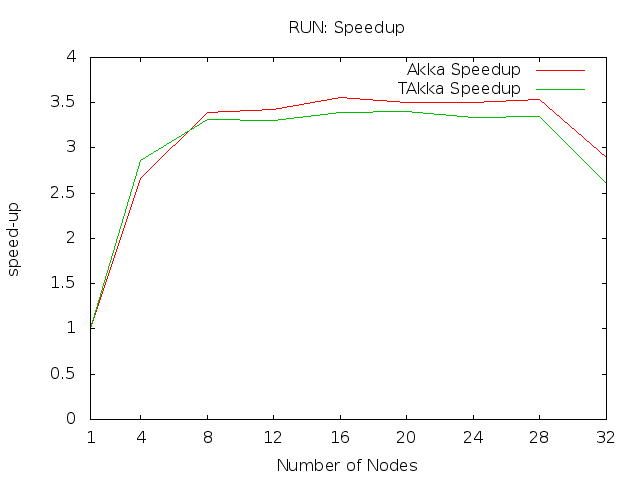
\includegraphics[scale=0.16]{RUN_speedup.png}
        }
        \subfigure[]{
           \label{fig:2_16}
           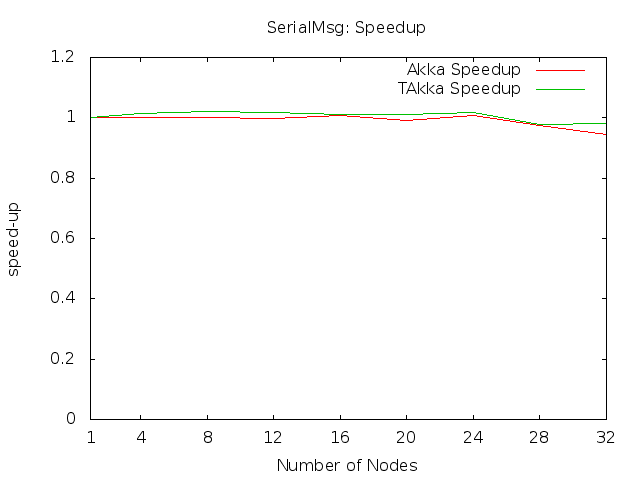
\includegraphics[scale=0.16]{SerialMsg_speedup.png}
        }\\        
    \end{center}
     \caption{Scalability Benchmarks 2}
   \label{scalability}
\end{figure}

